\documentclass[11pt]{beamer}
\usetheme{Antibes}
\usepackage[utf8]{inputenc}
\usepackage{amsmath}
\usepackage{amsfonts}
\usepackage{amssymb}
\usepackage{graphicx}
%\author{}
%\title{}
%\setbeamercovered{transparent} 
%\setbeamertemplate{navigation symbols}{} 
%\logo{} 
%\institute{} 
%\date{} 
%\subject{} 
\begin{document}

%\begin{frame}
%\titlepage
%\end{frame}

%\begin{frame}
%\tableofcontents
%\end{frame}
\section{Bestimmung der Schallgeschwindigkeit durch Laufzeitmessung}
\subsection{Versuchsbeschreibung}
\begin{frame}
\begin{itemize}
\item Bestimmung der Schallgeschwindigkeit in Luft:
\begin{equation*}
v=\frac{s}{t}
\end{equation*}
\item Für die Temperaturabhängigkeit gilt:
\begin{equation*}
v=v_0\cdot \sqrt{\frac{T}{T_0}} 
\end{equation*}
\end{itemize} 
\end{frame}
\subsection{Versuchsaufbau und Durchführung}
\begin{frame}
\begin{figure}[H]
\centering
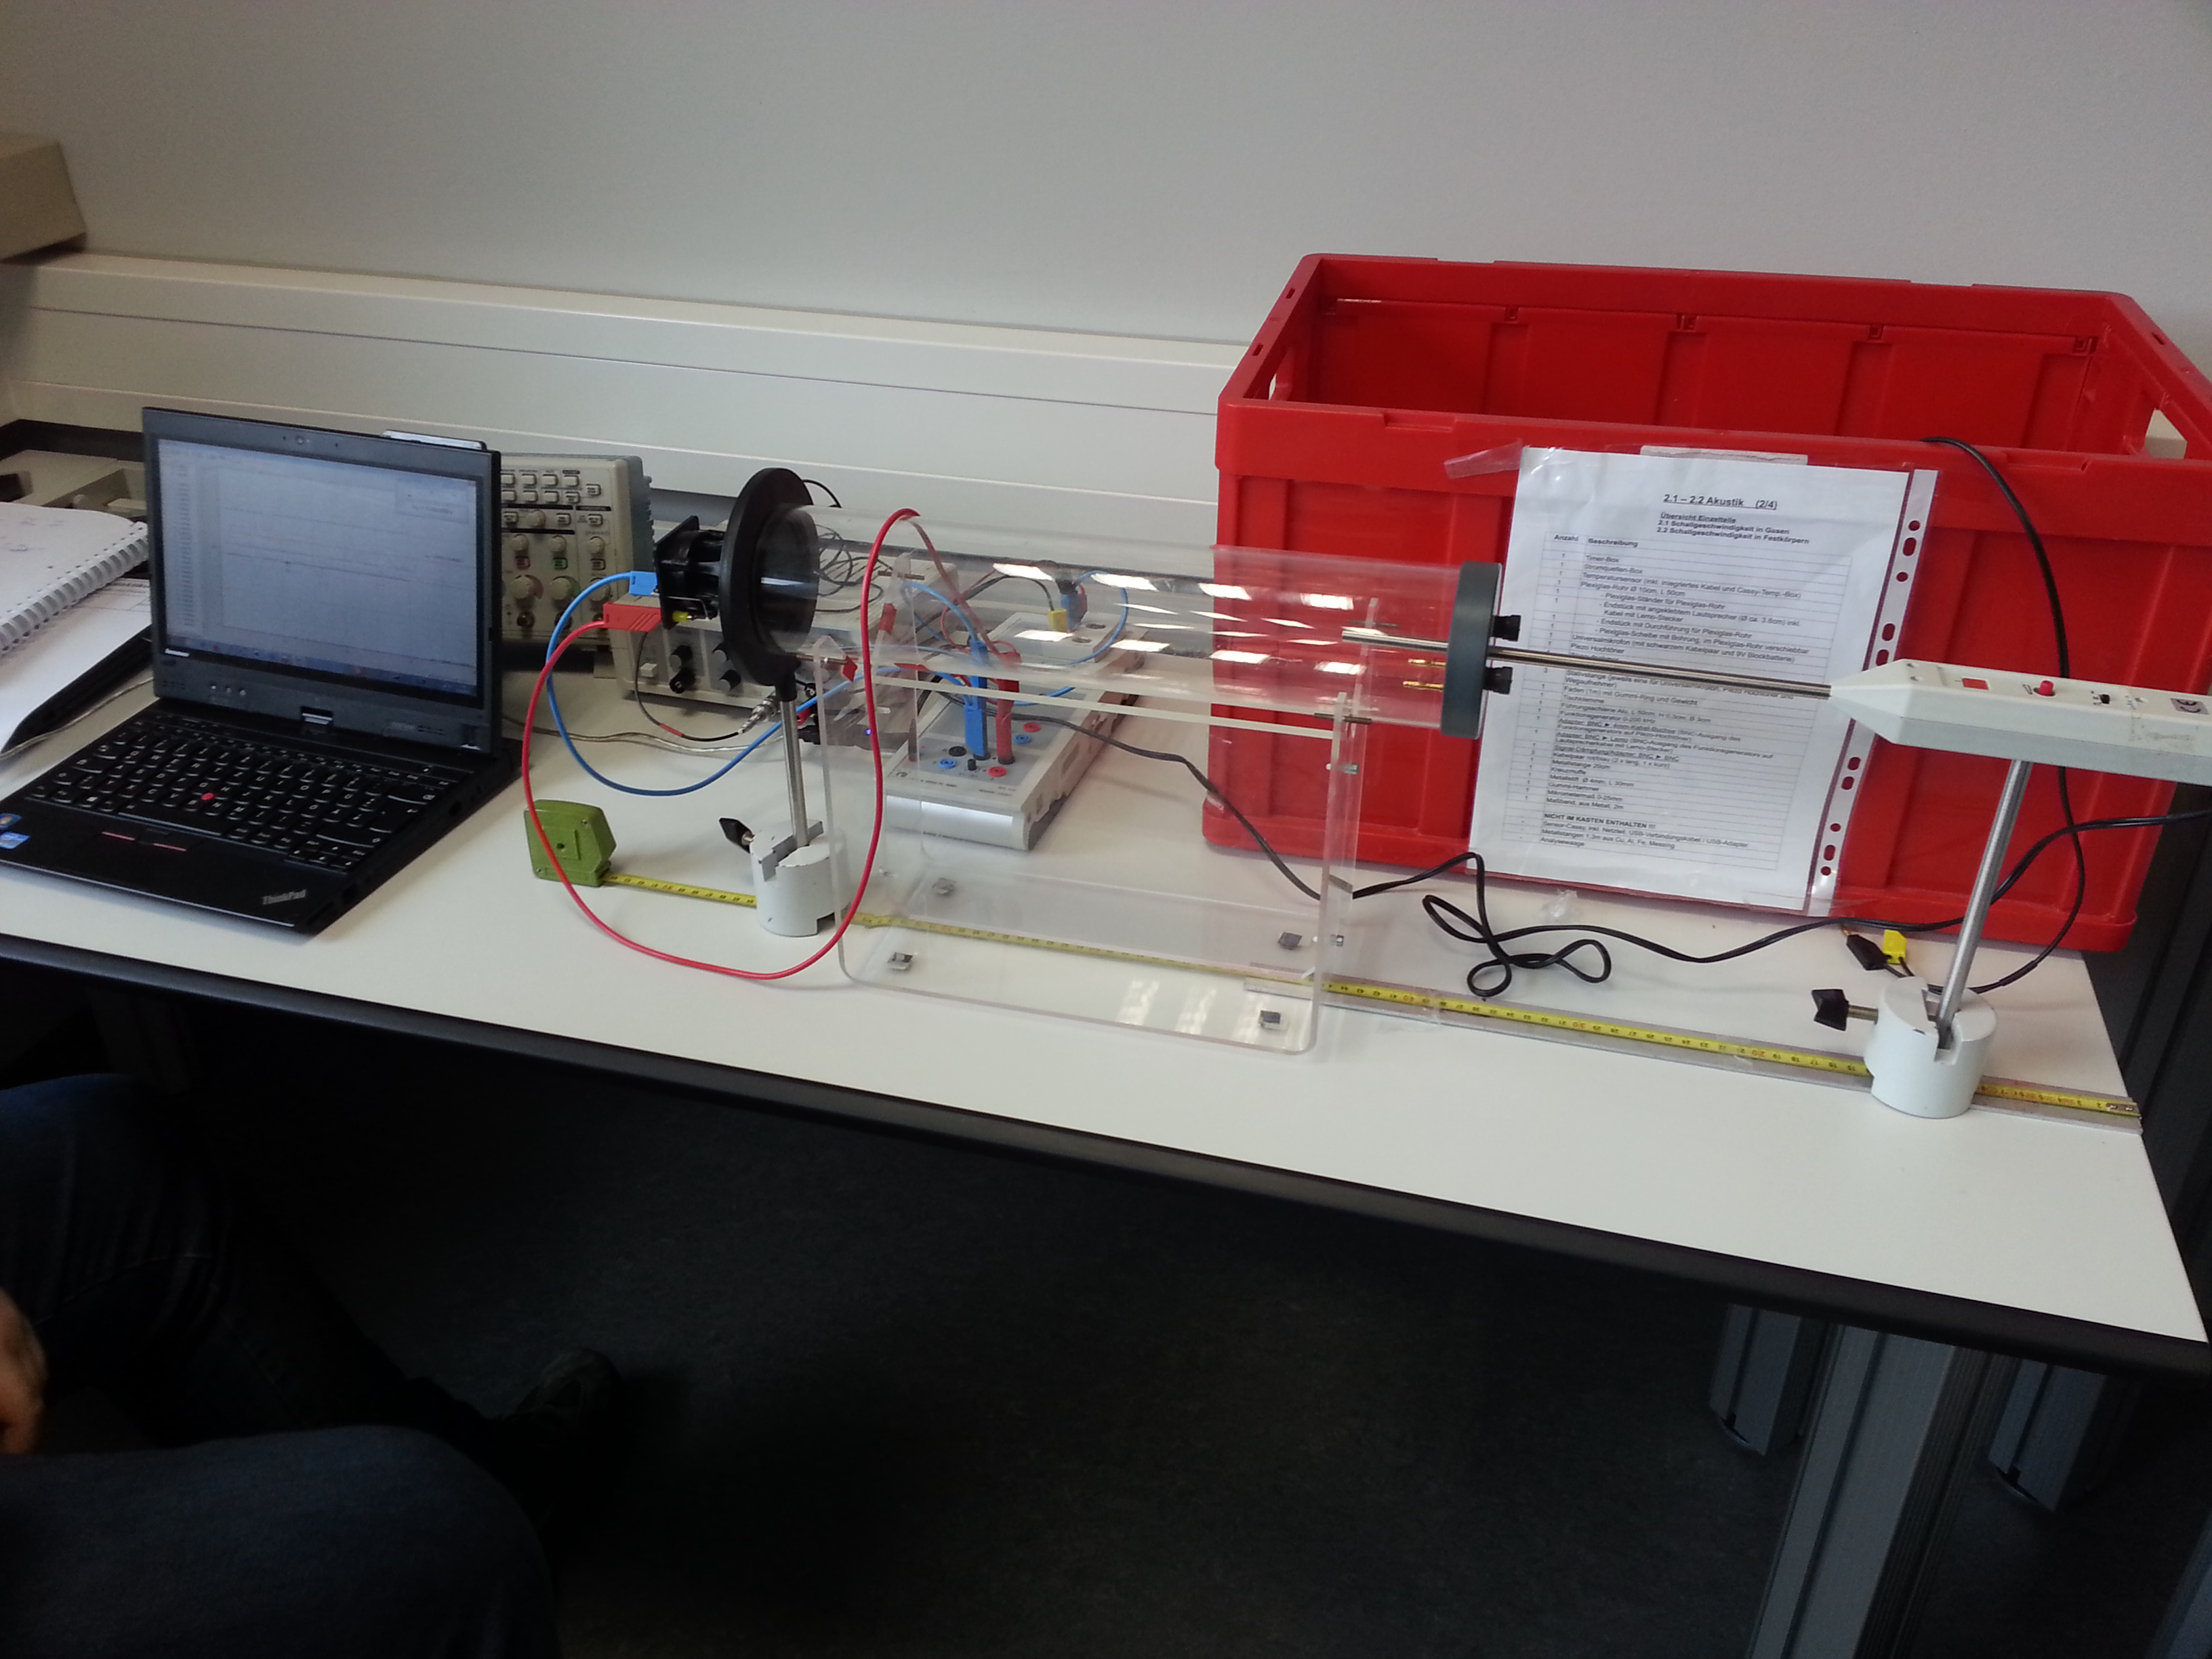
\includegraphics[scale=0.08]{Bilder/laufzeit-cassy.jpg}
\caption{Versuchsaufbau der Laufzeitmessung mit dem Sensor-Cassy.}
\end{figure}
\end{frame}
\subsection{Rohdaten}
\begin{frame}
\begin{figure}[H]
\centering
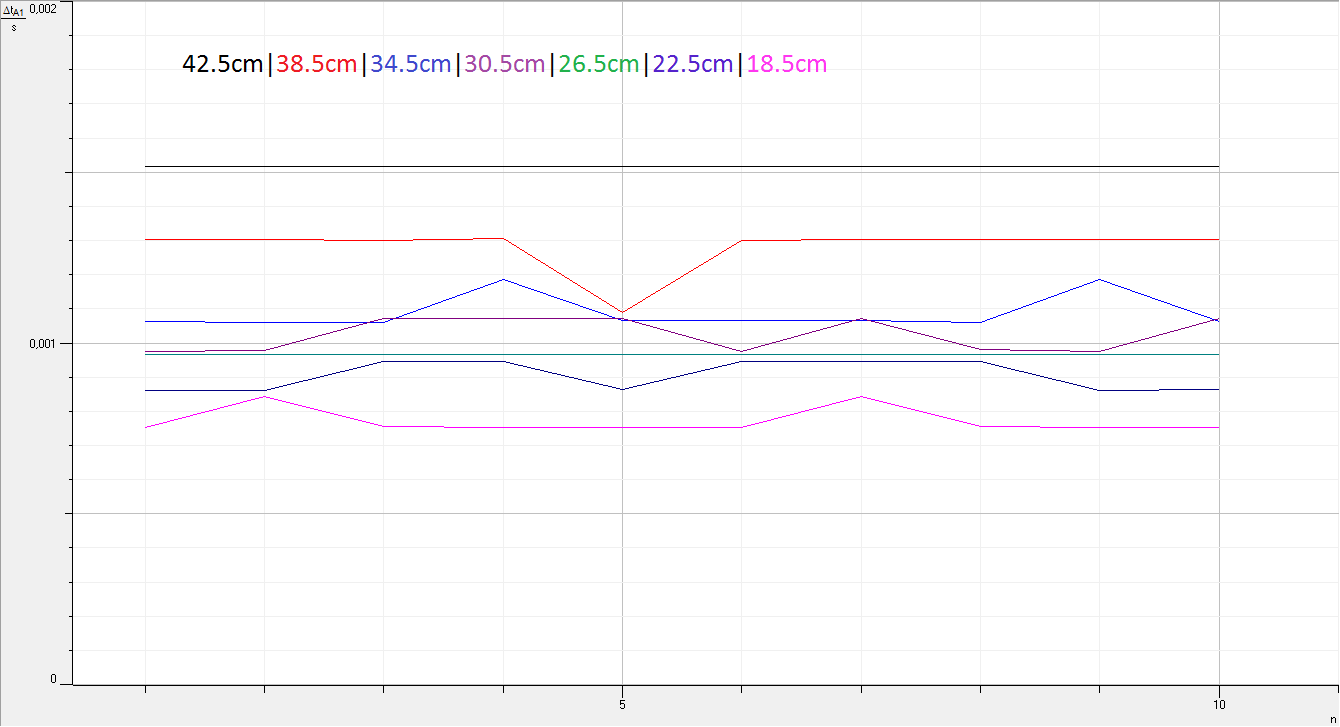
\includegraphics[scale=0.4]{Bilder/Rohdaten-Laufzeitmessung.png}
\caption{Beispiel einer Laufzeitmessung mit dem Sensor-Cassy bei verschiedenen Abständen}
\label{Laufzeitrohdaten}
\end{figure}
\end{frame}
\begin{frame}
\begin{figure}[H]
\centering
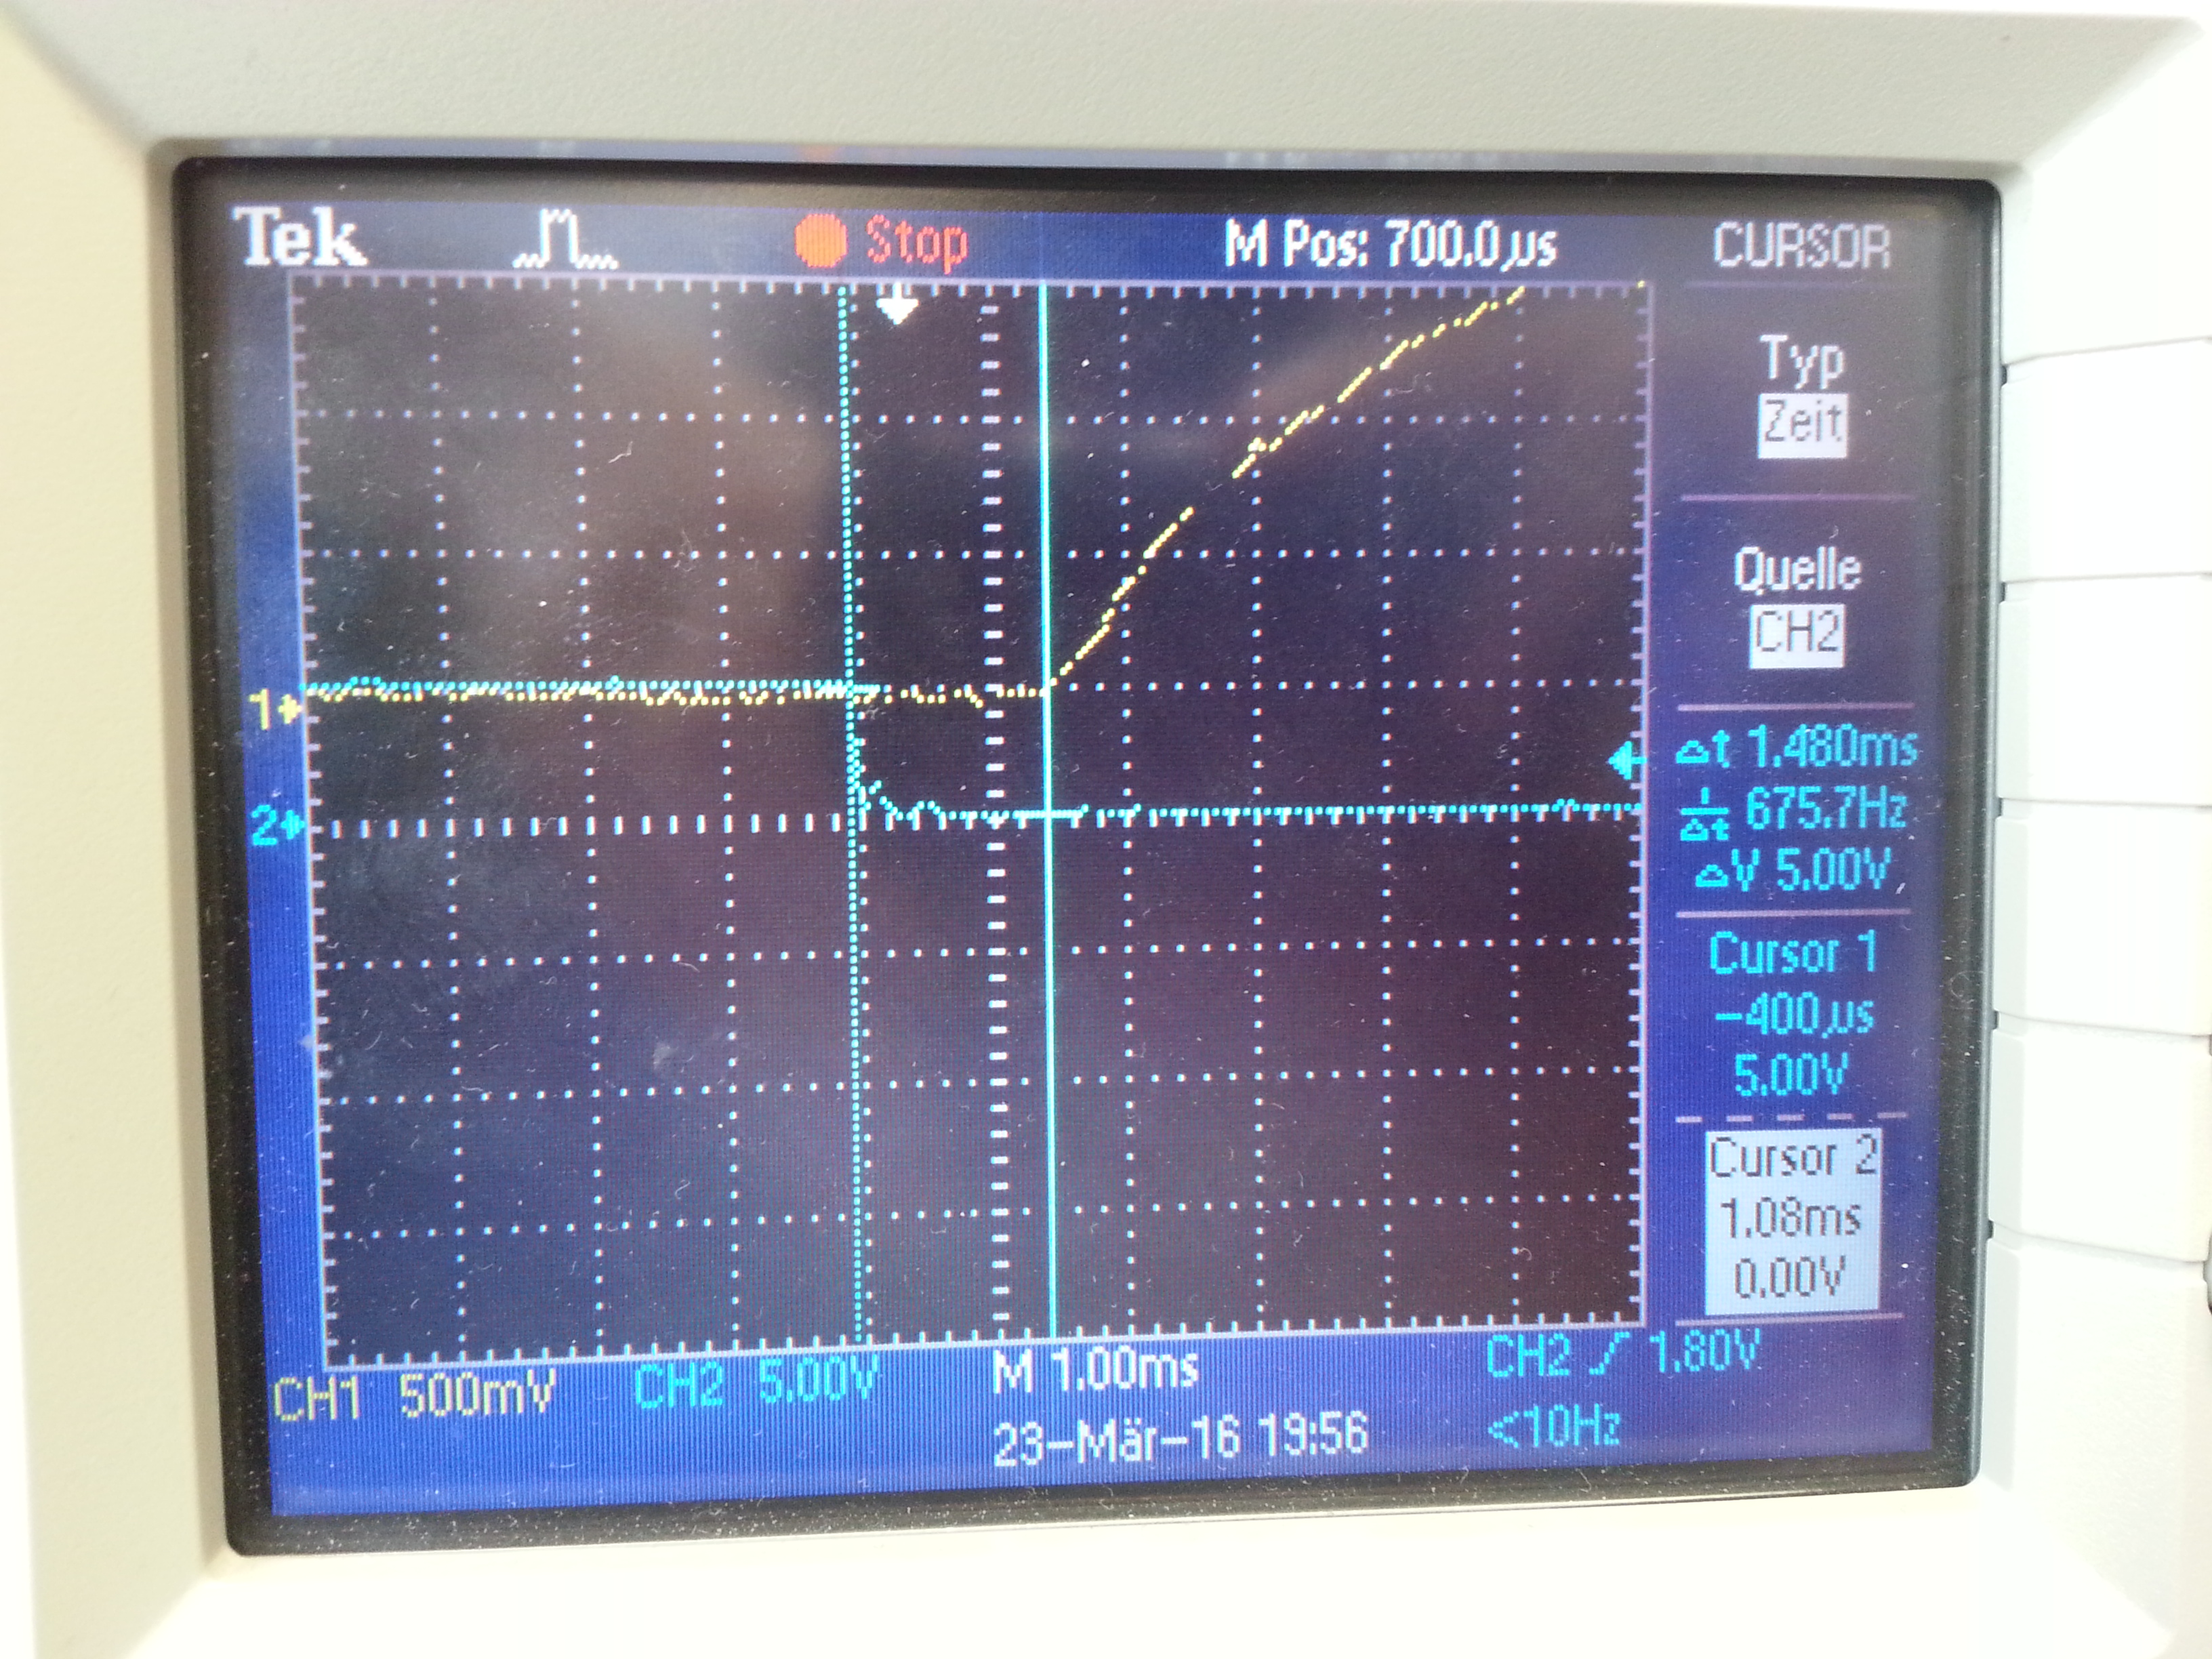
\includegraphics[scale=0.08]{Bilder/oszi.jpg}
\caption{Beispiel einer Laufzeitmessung mit dem Oszilloskop bei einem Abstand von 42.5cm}
\end{figure}
\end{frame}
\begin{frame}
\begin{table}[H]\centering
\caption{Werte der Laufzeitmessung mit dem Oszilloskop}
\begin{tabular}{c|c}
Abstand in m & Zeitdifferenz der Spannungspeaks in ms\\ 
\hline
$42.5$& $1.48$\\ 
$34.5$& $1.24$\\
$26.5$& $1.08$\\
\end{tabular} 
\end{table}
\begin{itemize}
\item $\sigma_t=0.04ms$
\item $T=22.6^{\circ}$
\end{itemize}
\end{frame}
\subsection{Transformation der Rohdaten/Analyse}
\begin{frame}
\begin{table}[H]\centering
\caption{Mittelwerte der Cassy-Laufzeitmessung mit Fehlern}
\begin{tabular}{c|c|c}
Abstand in m & Mittelwert der Zeit in ms & $\sigma_t$ in ms\\ 
\hline
$42.5$& $1.51705$& $4.104 \cdot 10^{-4}$\\ 
$38.5$& $1.28692$& $7.141 \cdot 10^{-2}$\\
$34.5$& $1.08284$& $4.526 \cdot 10^{-2}$\\
$30.5$& $1.05089$& $4.390 \cdot 10^{-2}$\\
$26.5$& $0.96639$& $5.193 \cdot 10^{-4}$\\
$22.5$& $0.92490$& $3.756 \cdot 10^{-2}$\\
$18.5$& $0.80627$& $4.416 \cdot 10^{-2}$\\
\end{tabular} 
\end{table}
\end{frame}
\begin{frame}
\begin{figure}[H]
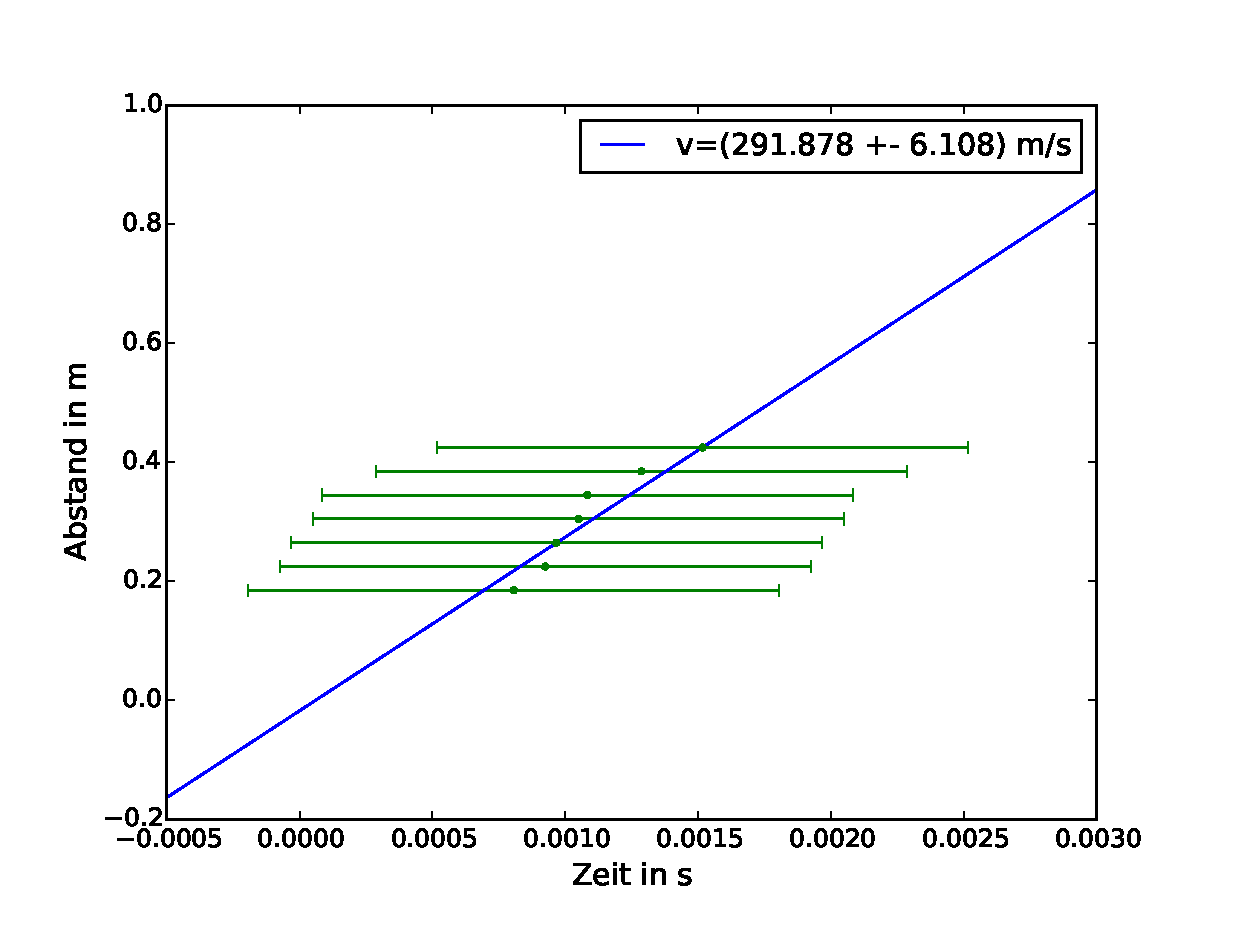
\includegraphics[scale=0.3]{Bilder/Linreg-Laufzeit.eps}
%\caption{Lineare Regression durch die Mittelwerte der Cassy-Messung mit ihren Fehlern}
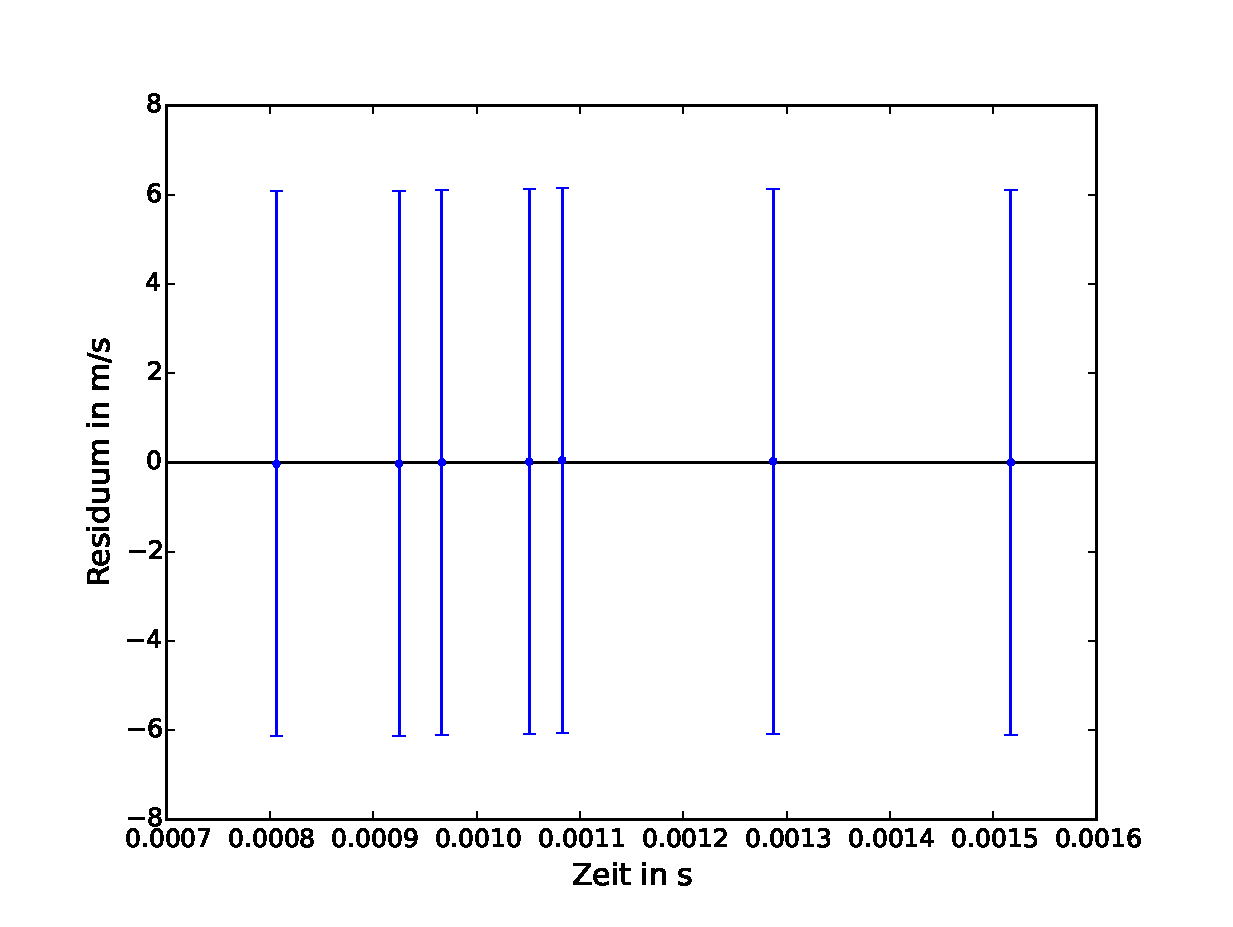
\includegraphics[scale=0.3]{Bilder/Residuen-Laufzeit.eps}
%\caption{Residuen des Fits, der Cassy-Messung}
\end{figure}
\begin{itemize}
\item $\chi^2$ pro Freiheitsgrad $=5.677$
\end{itemize}
\end{frame}
\begin{frame}
\begin{figure}[H]
\centering
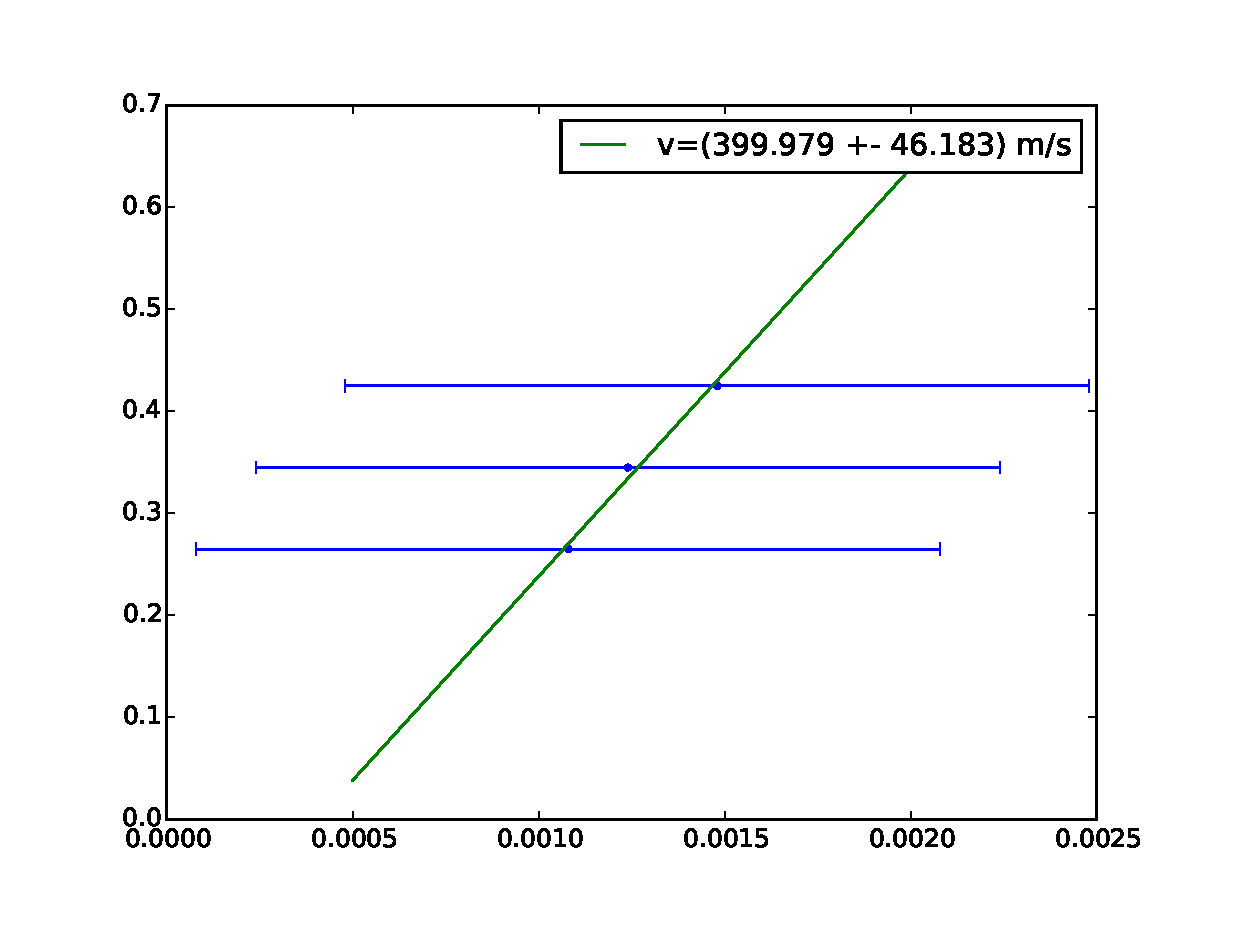
\includegraphics[scale=0.3]{Bilder/Linreg-Oszi.eps}
%\caption{$\chi^2$ pro Freiheitsgrad $=0.664$}
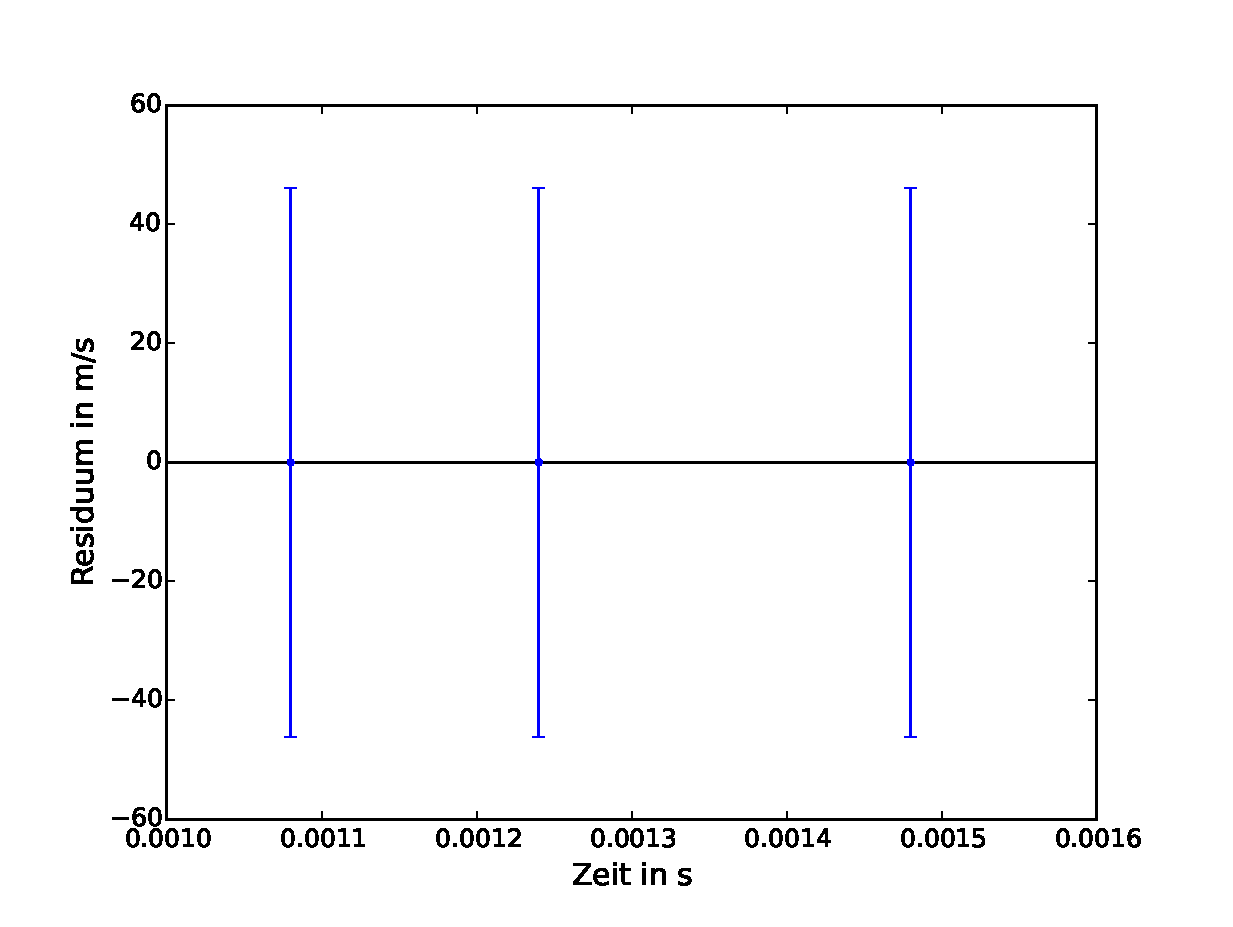
\includegraphics[scale=0.3]{Bilder/Residuen-Oszi.eps}
%\caption{Residuen des Fits der Oszilloskop-Messung}
\end{figure}
\begin{itemize}
\item $\chi^2$ pro Freiheitsgrad $=0.664$
\end{itemize}
\end{frame}
\subsection{Fazit}
\begin{frame}
\begin{itemize}
\item Literaturwert: $344.98 \, \frac{m}{s}$
\item Cassy: $v=(291.878 \pm 6.108) \frac{m}{s} \rightarrow 8\sigma$ Abweichung
\item Oszilloskop: $v=(399.979 \pm 46.183)\frac{m}{s}\rightarrow 1\sigma$ Abweichung
\end{itemize}
\end{frame}
\end{document}